\chapter{Methods\label{cha:methods}}
Data collection on flights through the airspace monitored and controlled by Isavia has been going on for several years now. This data is filtered and stored on company servers for reference and analysis. The statistical analysis for this project was done in Python and used to determine the fleet mix at BIKF, runway occupancy and landing intervals.

\section{Data collecting and data filtering}
The data collection comences on 21 November 2014 with the acceptance of the Automatic Dependent Surveillance-Broadcast (ADS-B) system by Isavia. ADS-B was preferred to radar at Keflavik Internetional Airport because of signal accuracy \cite{isavia_wiki}. The ADS-B equipped aircraft through Keflavik Airport is estimated around $90\%$ \cite{isavia-rounardeild_rannsoknir_2018}. The aircraft surveillance data specifications used for measurements are in the Eurocontrol ASTERIX Category 21 standard \cite{ASTERIX_ADS-B_specs}.
The reading from the position of the ADS-B antenna of the aircraft is used instead of the tail and nose positions. This simplification could result in a few seconds difference. Certain filtering of the ADS-B data is applied before commencing measurements and calculations: 
\begin{itemize}
    \item All records with no latitude, longitude and/or time data are omitted.
    \item The records are filtered with regards to quality, i.e. filtered with regards to Target Surveillance status, MOPS version, NUC/NIC, NACp, SIL and PIC.
    \item An ADS-B data record within 0.5 second from another is omitted, i.e. if there are less than 0.5 seconds between two successive locations one of the records is omitted.
    \item An algorithm is used to analyse the data and determine if it originates from two different flights (the flight stops for 15 minutes or more after/before taxiing). If so the data for the second flight is omitted
    \item The velocity is calculated from ADS-B location data and ADS-B time data (velocity = distance travelled/time). The ADS-B velocity record is optional in the ASTERIX category 21 standard and is therefore unreliable in measurements. Since the velocity is calculated from measured data, it can exhibit spikes. To get a more realistic velocity curve, a Savitzky-Golay filter is applied to smooth the data.
    \item An aircraft main gear lift-off is considered to be the point where the ADS-B ground bit is removed, i.e. the ADS-B ground bit goes from a value of 1 to a value of 0.
    \item An aircraft touchdown is considered to be the point where the ADS-B ground bit is set, i.e. the ADS-B ground bit goes from a value of 0 to a value of 1.
    \item An aircraft is considered to be stationary when the velocity is below 0.5 knots and to be moving if the velocity is greater than 0.5 knots.
    \cite{isavia_wiki}
\end{itemize}


\fxnote{The ROT measurements have been checked by: comparing them to measurements made by hand.
Who measures and who checks them and how???}

\section{Data manipulation}
The data was obtained from the database using SQL server and stored as csv files. The the manipulations on the data frames were performed using the functionality of Pandas and NumPy data analysis tools and computing packages for Python. A key table containing information about 2300 aircraft models, including ICAO and RECAT-EU wake turbulence categories for each model, was also used as reference. 
The reference table was provided by Eurocontrol. 
The Isavia aircraft data was cross-referenced with the Eurocontrol key table based on ICAO aircraft type labels, the mutual characteristic in both data sets. 
After cross-referencing a RECAT-EU category was assigned to each of the aircraft arriving at BIKF in peak hours. Outliers bellow the 0,003 quantile and above the 0,997 quantile were removed from data set based on AROTs. 
The resulting data frame was used for the analysis in this project. 
It contained over 11500 arrivals for the time period of almost four years (from 01.01.2015 til 30.11.2018). The data frame contained unique information about the AROT of each aircraft, the landing time and used runway, along with the ICAO wake category. 


\subsection{Aircraft traffic mix}

\fxnote{Looked at the traffic mix, pie chart and mix by model}\\

\begin{figure}[ht]
    \centering
    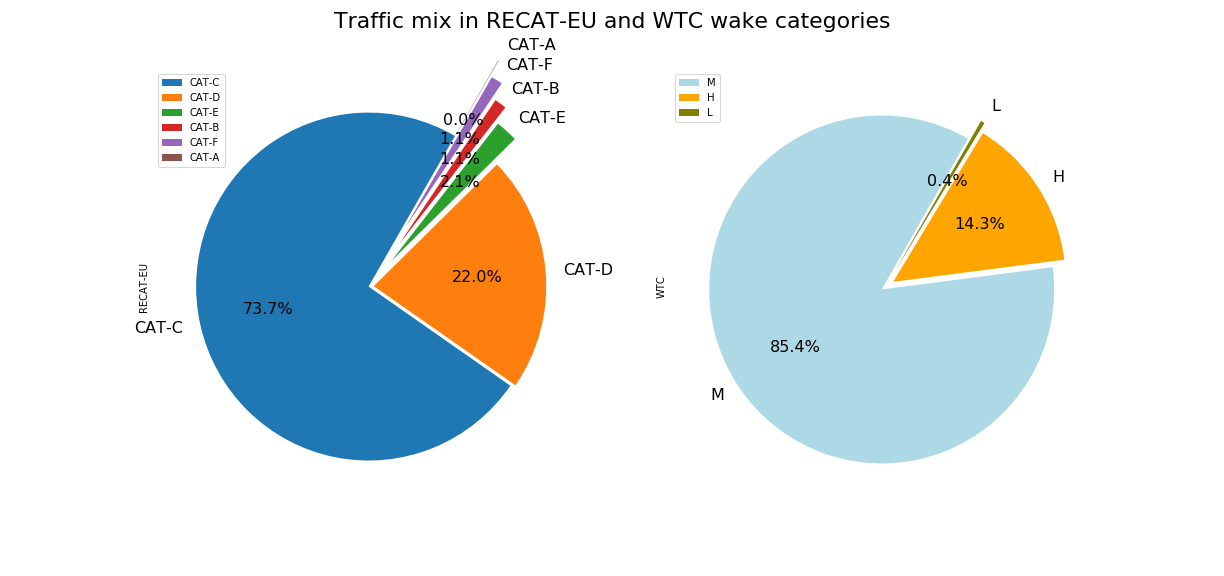
\includegraphics[width=1\textwidth]{graphics/fig_post_fast_exit_mix_pie_v2.png}
    \caption[Traffic mix in RECAT-EU and ICAO WTC]{The traffic mix at Keflavik Airport represented in RECAT-EU categories alongside ICAO WTC categories.}
    \label{fig:post_fast_exit_mix_pie_v2}
\end{figure}


\begin{figure}
    \centering
    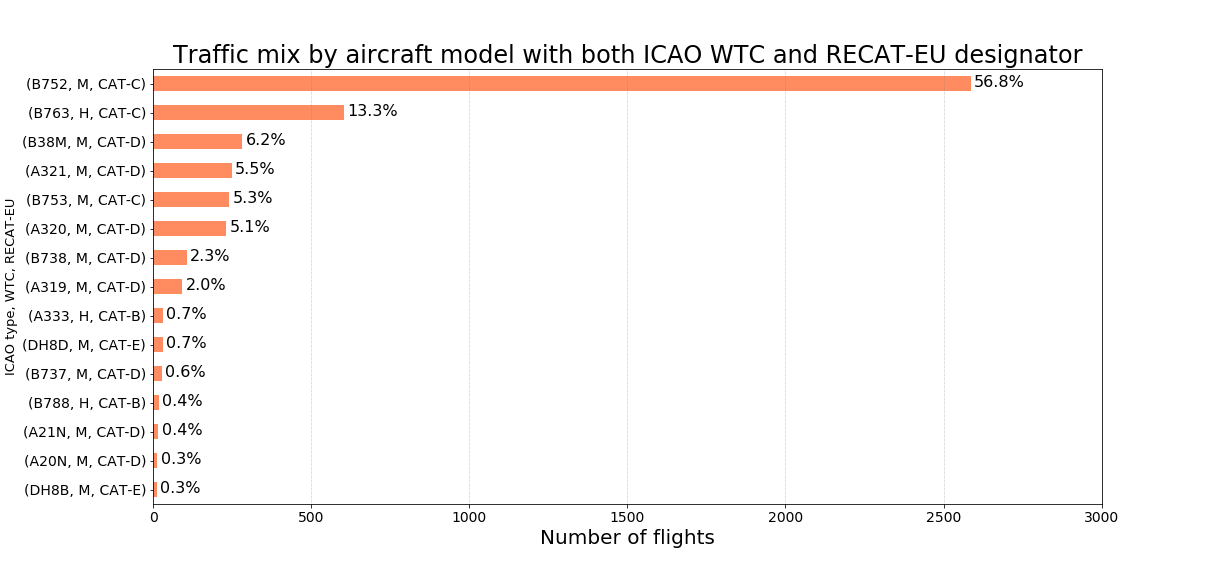
\includegraphics[width=1\textwidth]{graphics/fig_traffic_mix_by_model.png}
    \caption[Traffic mix by aircraft model.]{The traffic mix at Keflavik Airport grouped by aircraft model. The aircraft models are shown with their RECAT-EU and ICAO WTC designators}
    \label{fig:traffic_mix_by_model}
\end{figure}

% -----------------------
\subsection{Arrival runway occupancy times}

\begin{figure}
    \centering
    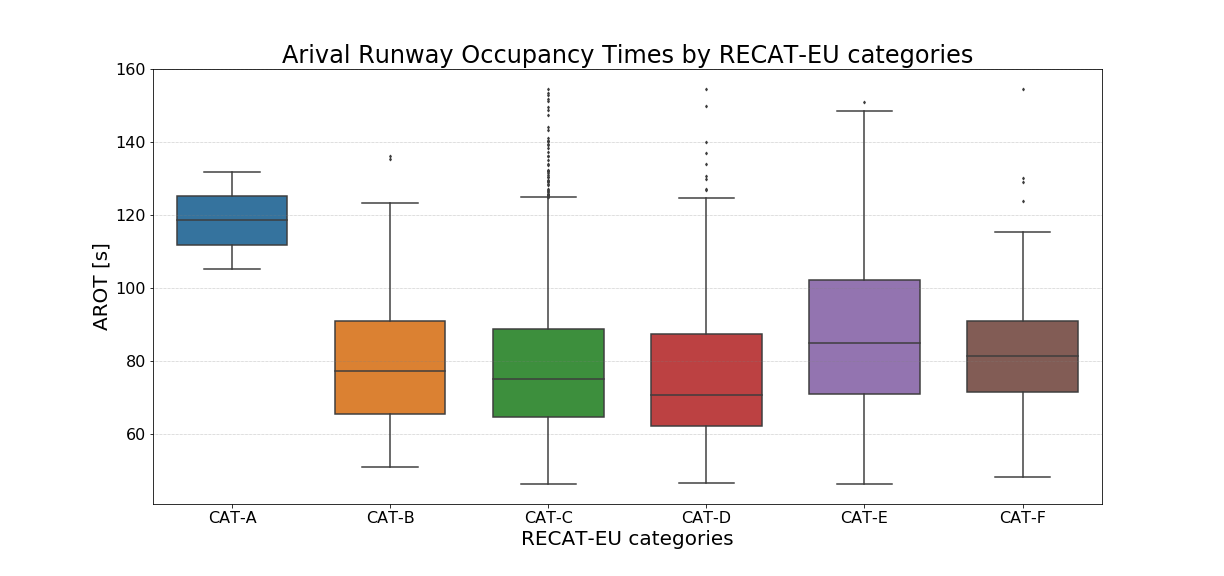
\includegraphics[width=1\textwidth]{graphics/fig_RECAT_AROTs_boxplot.png}
    \caption[AROTs boxplot for RECAT categories, all runways]{Arrival Runway Occupancy Times for the different RECAT-EU categories based on data gathered for a period of one year (since October, 2017). The box plot shows the AROTs for all runways at BIKF.}
    \label{fig:RECAT_AROTs_boxplot}
\end{figure}


% Please add the following required packages to your document preamble:
% \usepackage{graphicx}
\begin{table}[]
\centering
\resizebox{0.8\textwidth}{!}{%
\begin{tabular}{lr|r|r|r|r|r|r|r|}
\cline{3-9}
                          & \multicolumn{1}{c|}{}   & \multicolumn{7}{c|}{AROT [s]} \\ \hline
\multicolumn{1}{|l|}{RECAT-EU} & count & mean & std & min & 25\% & 50\% & 75\% & max \\ \hline
\multicolumn{1}{|l|}{CAT-A}    & 2     & 119  & 19  & 105 & 112  & 119  & 125  & 132 \\ \hline
\multicolumn{1}{|l|}{CAT-B}    & 53    & 81   & 20  & 51  & 65   & 77   & 91   & 136 \\ \hline
\multicolumn{1}{|l|}{CAT-C}    & 3436  & 78   & 17  & 46  & 65   & 75   & 89   & 155 \\ \hline
\multicolumn{1}{|l|}{CAT-D}    & 1029  & 75   & 18  & 46  & 62   & 71   & 87   & 155 \\ \hline
\multicolumn{1}{|l|}{CAT-E}    & 95   & 88   & 24  & 46  & 71   & 85   & 101  & 151 \\ \hline
\multicolumn{1}{|l|}{CAT-F}    & 49    & 84   & 22  & 48  & 72   & 81   & 91   & 155 \\ \hline
\end{tabular}%
}
\caption[AROTs for the air traffic mix by RECAT]{AROT statistics for the air traffic mix at KEF by RECAT-EU categories. The count is the number of landings in peak hours since October 2017}
\label{tab:AROT_RECAT_stats}
\end{table}


% Please add the following required packages to your document preamble:
% \usepackage{graphicx}
\begin{table}[]
\centering
\resizebox{0.8\textwidth}{!} & \multicolumn{1}{l|}{50\%} & \multicolumn{1}{l|}{75\%} & \multicolumn{1}{l|}{max} \\ \hline
\multicolumn{1}{|l|}{SUMMER} & \multicolumn{1}{r|}{3727} & 76  & 17 & 46 & 63  & 72 & 87  & 155 \\ \hline
\multicolumn{1}{|l|}{WINTER} & \multicolumn{1}{r|}{937}  & 84  & 20 & 45 & 69  & 84 & 96  & 153 \\ \hline
\end{tabular}%
}
\caption[AROTs for the air traffic mix by season]{AROT statistics for the air traffic mix at KEF by season. The count is the number of landings in peak hours since October 2017}
\label{my-label2}
\end{table}

% Please add the following required packages to your document preamble:
% \usepackage{graphicx}
\begin{table}[]
\centering
\resizebox{0.8\textwidth}{!} & \multicolumn{1}{l|}{50\%} & \multicolumn{1}{l|}{75\%} & \multicolumn{1}{l|}{max} \\ \hline
\multicolumn{1}{|l|}{RWY 01} & 963 & 85 & 21 & 46 & 68 & 88 & 100 & 152 \\ \hline
\multicolumn{1}{|l|}{RWY 10} & 852 & 85 & 11 & 61 & 78 & 84 & 91 & 155 \\ \hline
\multicolumn{1}{|l|}{RWY 19} & 1511 & 67 & 10 & 46 & 61 & 66 & 71 & 155 \\ \hline
\multicolumn{1}{|l|}{RWY 28} & 401 & 68 & 14 & 49 & 60 & 66 & 72 & 155 \\ \hline
\end{tabular}%
}
\caption[AROTs for the air traffic mix by runway for the summer]{AROT statistics for the air traffic mix at KEF by runway for the summer of 2018. The count is the number of landings in peak hours.}
\label{my-label3}
\end{table}


% Please add the following required packages to your document preamble:
% \usepackage{graphicx}
\begin{table}[]
\centering
\resizebox{0.8\textwidth}{!} & \multicolumn{1}{l|}{50\%} & \multicolumn{1}{l|}{75\%} & \multicolumn{1}{l|}{max} \\ \hline
\multicolumn{1}{|l|}{RWY 01} & 284 & 88 & 26 & 47 & 63 & 90 & 106 & 153 \\ \hline
\multicolumn{1}{|l|}{RWY 10} & 333 & 93 & 12 & 70 & 85 & 91 & 99 & 144 \\ \hline
\multicolumn{1}{|l|}{RWY 19} & 251 & 72 & 12 & 51 & 65 & 70 & 75 & 140 \\ \hline
\multicolumn{1}{|l|}{RWY 28} & 69 & 73 & 13 & 49 & 63 & 72 & 79 & 105 \\ \hline
\end{tabular}%
}
\caption[AROTs for the air traffic mix by runway for the winter]{AROT statistics for the air traffic mix at KEF by runway for the winter season. The count is the number of landings in peak hours since October 2017}
\label{my-label4}
\end{table}


% Please add the following required packages to your document preamble:
% \usepackage{graphicx}
% \usepackage[table,xcdraw]{xcolor}
% If you use beamer only pass "xcolor=table" option, i.e. \documentclass[xcolor=table]{beamer}
\begin{table}[]
\centering
\resizebox{0.8\textwidth}{!} & \multicolumn{1}{l|}{50\%} & \multicolumn{1}{l|}{75\%} & \multicolumn{1}{l|}{max} \\ \hline
\rowcolor[HTML]{DAE8FC} 
\multicolumn{1}{|l|}{\cellcolor[HTML]{DAE8FC}January} & 95 & 86 & 20 & 54 & 70 & 85 & 96 & 136 \\ \hline
\rowcolor[HTML]{DAE8FC} 
\multicolumn{1}{|l|}{\cellcolor[HTML]{DAE8FC}February} & 80 & 87 & 16 & 52 & 75 & 86 & 93 & 144 \\ \hline
\rowcolor[HTML]{DAE8FC} 
\multicolumn{1}{|l|}{\cellcolor[HTML]{DAE8FC}March} & 215 & 84 & 18 & 47 & 70 & 85 & 95 & 150 \\ \hline
\rowcolor[HTML]{DAE8FC} 
\multicolumn{1}{|l|}{\cellcolor[HTML]{DAE8FC}April} & 221 & 82 & 17 & 47 & 69 & 81 & 93 & 139 \\ \hline
\rowcolor[HTML]{FFFC9E} 
\multicolumn{1}{|l|}{\cellcolor[HTML]{FFFC9E}May} & 386 & 75 & 13 & 46 & 67 & 74 & 83 & 140 \\ \hline
\rowcolor[HTML]{FFFC9E} 
\multicolumn{1}{|l|}{\cellcolor[HTML]{FFFC9E}June} & 647 & 73 & 16 & 47 & 62 & 68 & 80 & 155 \\ \hline
\rowcolor[HTML]{FFFC9E} 
\multicolumn{1}{|l|}{\cellcolor[HTML]{FFFC9E}July} & 729 & 72 & 16 & 46 & 61 & 68 & 77 & 155 \\ \hline
\rowcolor[HTML]{FFFC9E} 
\multicolumn{1}{|l|}{\cellcolor[HTML]{FFFC9E}August} & 724 & 80 & 18 & 46 & 64 & 81 & 91 & 148 \\ \hline
\rowcolor[HTML]{FFFC9E} 
\multicolumn{1}{|l|}{\cellcolor[HTML]{FFFC9E}September} & 632 & 78 & 18 & 46 & 64 & 75 & 88 & 152 \\ \hline
\rowcolor[HTML]{FFFC9E} 
\multicolumn{1}{|l|}{\cellcolor[HTML]{FFFC9E}October} & 609 & 79 & 17 & 46 & 66 & 76 & 91 & 155 \\ \hline
\rowcolor[HTML]{DAE8FC} 
\multicolumn{1}{|l|}{\cellcolor[HTML]{DAE8FC}November} & 220 & 84 & 23 & 48 & 66 & 82 & 99 & 151 \\ \hline
\rowcolor[HTML]{DAE8FC} 
\multicolumn{1}{|l|}{\cellcolor[HTML]{DAE8FC}December} & 106 & 87 & 23 & 51 & 69 & 86 & 99 & 153 \\ \hline
\end{tabular}%
}
\caption[AROTs for the air traffic mix by month]{AROT statistics for the air traffic mix at KEF by month. The count is the number of landings in peak hours since October 2017}
\label{my-label5}
\end{table}



\fxnote{Looked ar ROT, boxplot, seasonal and by RWY, fast exit effect}\\



% ---------------------------
\subsection{Landing time intervals}

\fxnote{Looked at LTI}\\


%\lipsum[14-20]
%%% Local Variables: 
%%% mode: latex
%%% TeX-master: "DEGREE-NAME-YEAR"
%%% End: 
